% Chapter Template

\chapter{Methodology} % Main chapter title

\label{Methodology} % Change X to a consecutive number; for referencing this chapter elsewhere, use \ref{ChapterX}

%----------------------------------------------------------------------------------------
%	SECTION 1
%----------------------------------------------------------------------------------------

\section{Sarosh's Perceptron Networks (SPNs)}

This chpater introduces the theoretical framework for Sarosh's Perceptron Networks (SPNs), designed to eliminate restrictions on neuron connectivity. The goal is to allow any two neurons to connect, forming a directed acyclic graph (DAG) like network (since cycles would cause deadlocks). This framework seeks to enhance neural networks by improving their connectivity while minimizing the associated increases in time and space complexities.
 
In theory, SPNs treat neurons as individual objects that can process inputs independently. These neurons may still depend on either the input data or other neurons for input, but the framework enables greater flexibility in forming connections across the network. Figure \ref{fig:exampleSPN} illustrates an arbitrary eample of such a network.

\begin{figure}[h!]
\centering
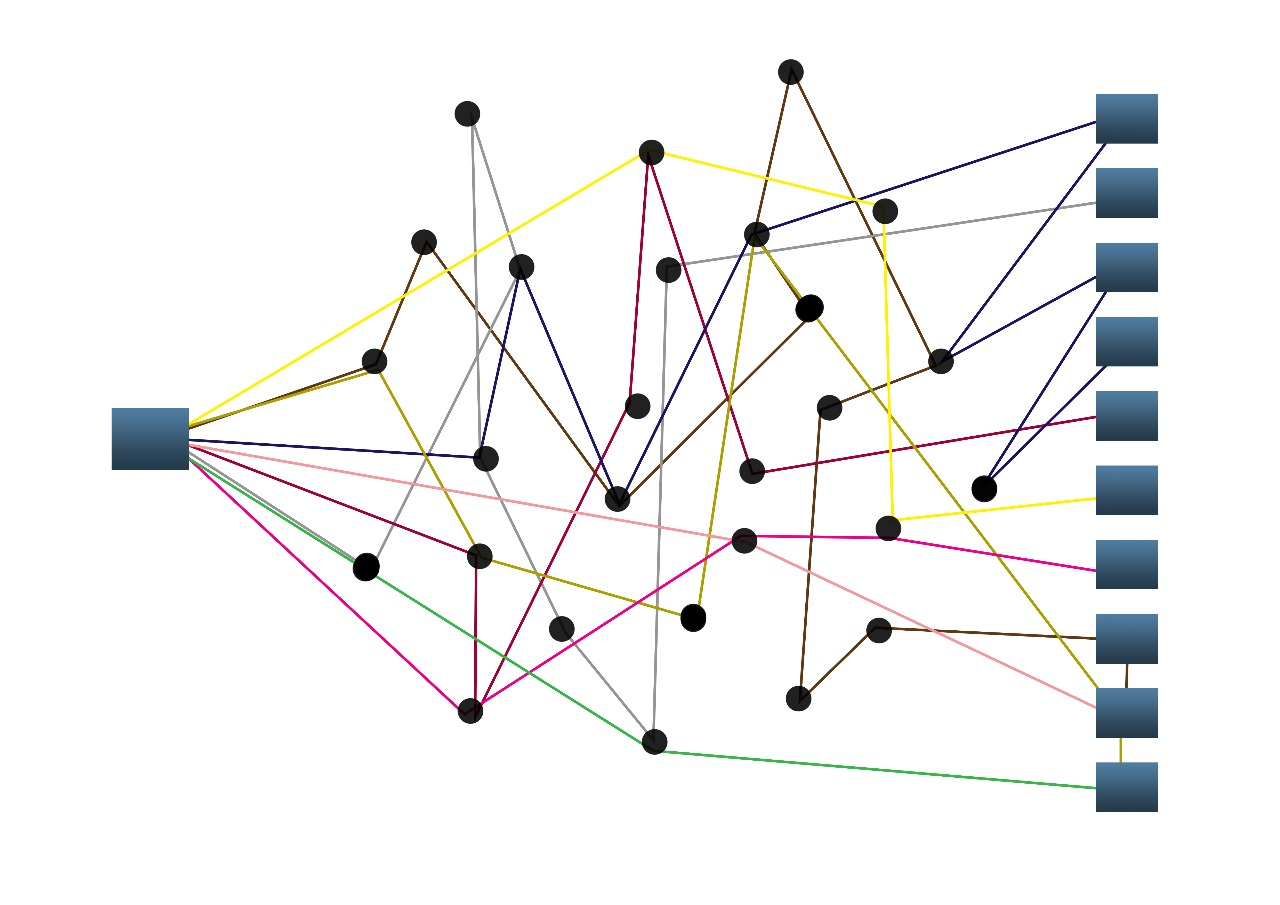
\includegraphics[width=0.7\textwidth]{Figures/Methodology/example_spn.jpg}
\caption{An Example SPN Network.}
\label{fig:exampleSPN}
\end{figure}

%-----------------------------------
%	SUBSECTION 1
%-----------------------------------
\subsection{Connection vs Neuron}

Before defining connectivity, it is important to clarify what is meant by a \emph{connection}. As illustrated in Figure \ref{fig:perceptronArch}, a perceptron (used interchangeably with "neuron" throughout this thesis) receives multiple inputs, each of which is assigned a learnable weight. The perceptron computes a weighted sum of its inputs, adds a learnable bias term, and passes the result through an activation function. In this thesis, a \textbf{connection} is defined as any instance where an input transmits its value to a given perceptron. Each connection introduces a new learnable weight parameter for that perceptron, thereby increasing the overall parameter count of the network by one per connection.

\begin{figure}[h!]
\centering
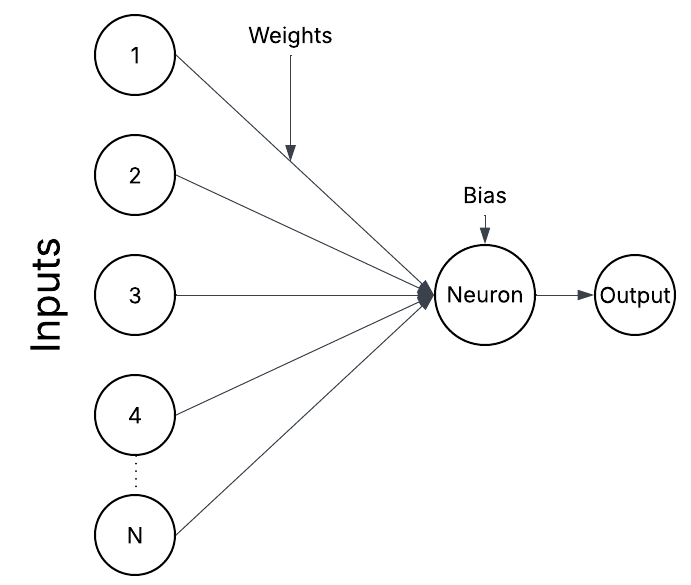
\includegraphics[width=0.4\textwidth, height=0.2\textheight]{Figures/Methodology/perceptron_architecture.png}
\caption{Architecture of a single Perceptron.}
\label{fig:perceptronArch}
\end{figure}

Accordingly, a Multi-Layer Perceptron is defined as a network composed of multiple layers of perceptrons. Thus, SPNs focuses on increasing the connection density of MLP models, while retaining the original number of neurons.

\subsection{Motivation for SPNs}

As illustrated in Figure \ref{fig:mlpStructure}, a typical MLP architecture features sequential connectivity: every neuron in a given layer is fully connected to all neurons in the subsequent layer. However, this conventional design omits two important types of connections.

\begin{figure}[h!]
\centering
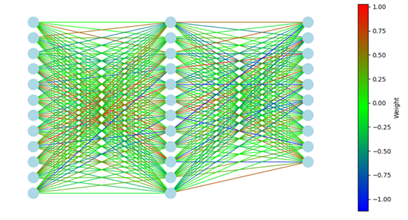
\includegraphics[width=0.7\textwidth]{Figures/Methodology/mlp_structural_diagram.png}
\caption{Low level illustration of an MLP.}
\label{fig:mlpStructure}
\end{figure}


\begin{enumerate}
    \item \textbf{Cross-layer connections} (shown in Figure \ref{fig:crossLayerConnection}): These connections would allow a layer to link to any preceding layer, not just the one immediately behind it.
    \begin{figure}[h!]
    \centering
    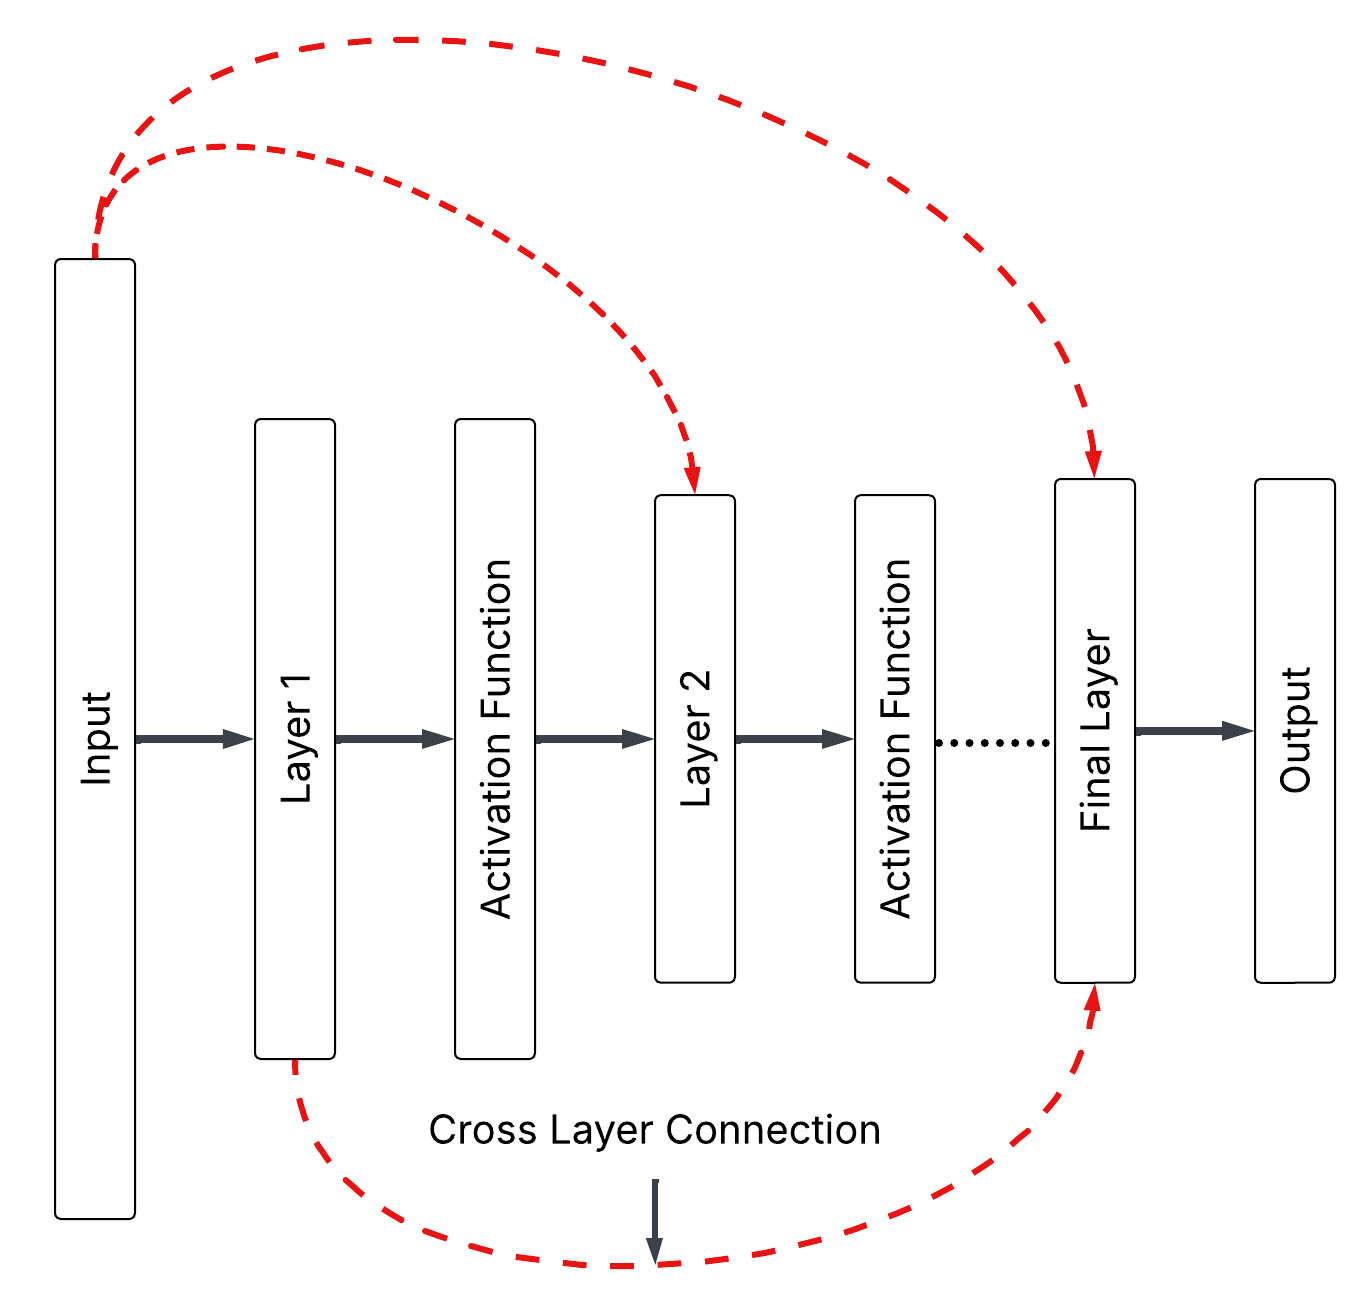
\includegraphics[width=0.7\textwidth]{Figures/Methodology/cross_layer_connections.png}
    \caption{Missing cross layer connections in MLP.}
    \label{fig:crossLayerConnection}
    \end{figure}

    \item \textbf{Intra-layer connections} (depicted in Figure \ref{fig:intraLayerConnection}): These would enable neurons within the same layer to connect to each other, a feature absent in standard MLPs.
    
    \begin{figure}[h!]
    \centering
    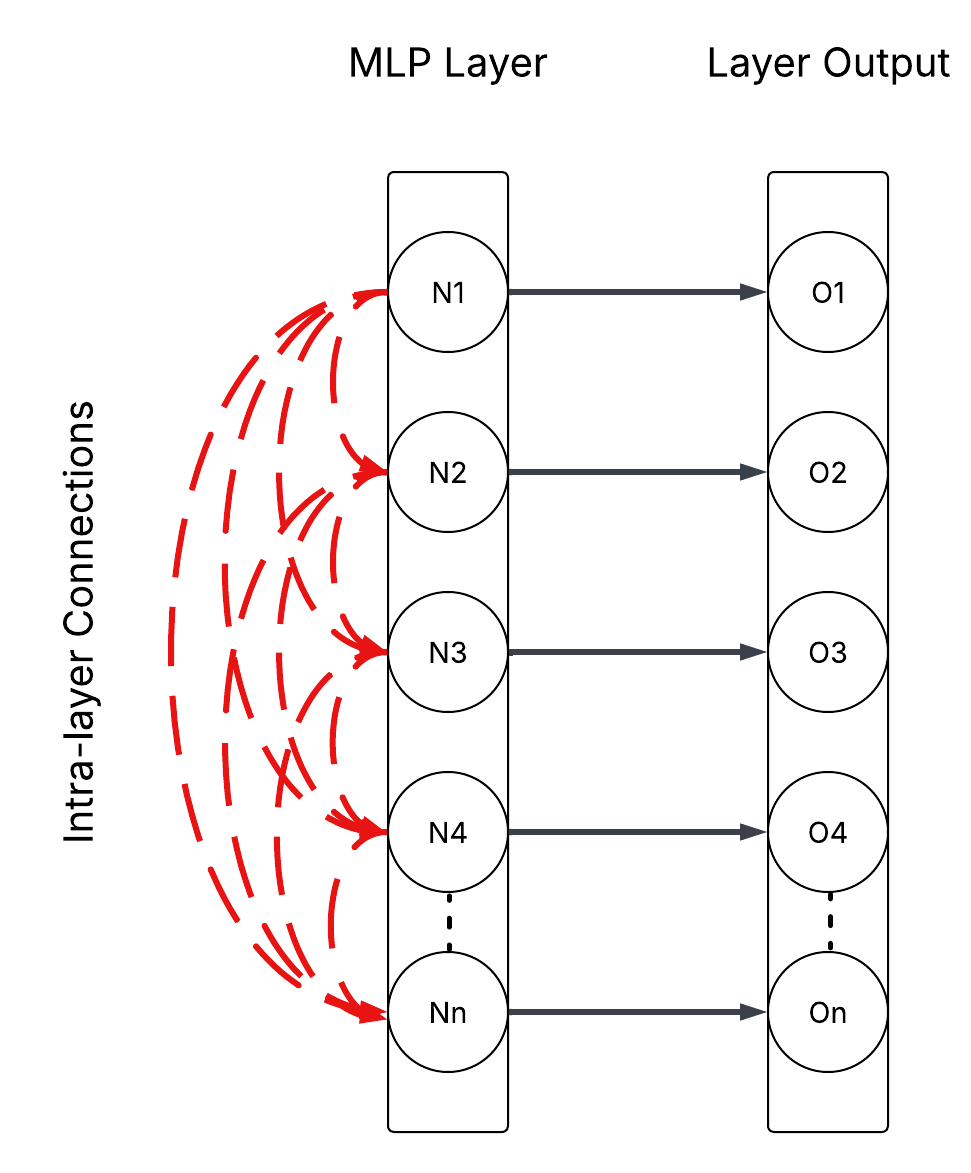
\includegraphics[width=0.5\textwidth, height=0.4\textheight]{Figures/Methodology/intra_layer_connections.png}
    \caption{Missing Intra-layer connections in a single MLP layer.}
    \label{fig:intraLayerConnection}
\end{figure}

\end{enumerate}

Alternatively, the weights of an MLP can be represented as a single, large weight matrix, where the x-axis corresponds to the input features and the y-axis to the neurons containing these weights, as illustrated in Figure \ref{fig:mlpWeights}. In the illustration, every layer is assumed to compose of only two neurons. 

\begin{figure}[h!]
\centering
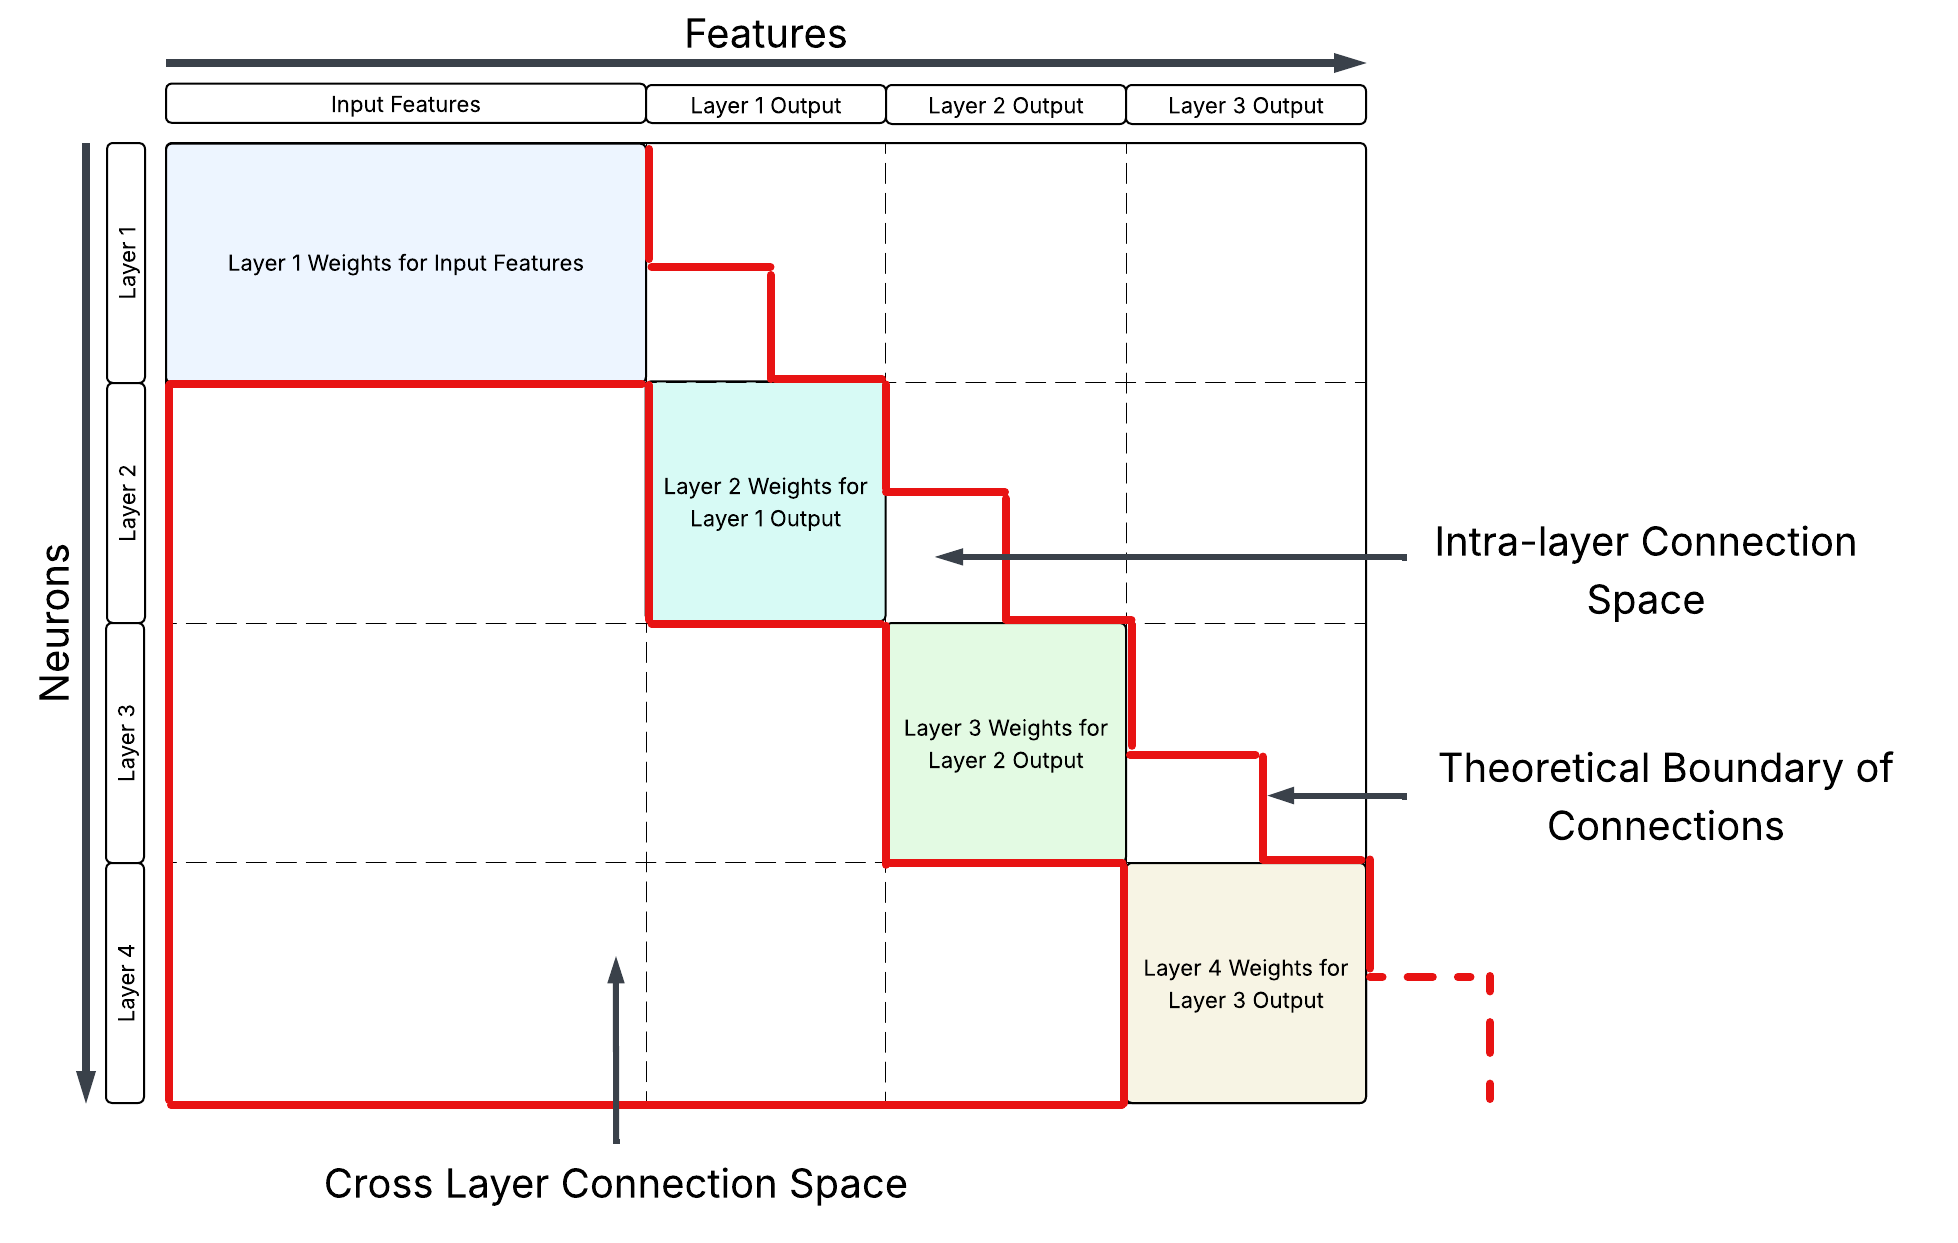
\includegraphics[width=1.0\textwidth]{Figures/Methodology/mlp_weight_matrix.png}
\caption{Cross Layer Connection Space and Intra-layer connection space with the theoretical connection boundary in the combined weight matrix of a traditiona MLP, assuming each layer has two neurons.}
\label{fig:mlpWeights}
\end{figure}

In this representation, the nonzero weights appear in diagonal arragned blocks, forming a staircase-like pattern that is separated along both axes. On the right side of the boxes, there is a theoretical boundary of connections. If any connections cross this boundary, it would form a cycle within the network where a neuron would be connected to itself (dependent on its own output). Thus, this boundary can never be crossed.

This visualization also makes it evident that both the left and right regions outside the blocks are completely empty. The empty region on the left corresponds to the absence of cross-layer connections, while the empty region on the right reflects the lack of intra-layer connections within the same layer.

Examining the weight matrix further, we notice that the right side of the matrix effectively determines the model’s number of layers. If we begin populating this region by introducing intra-layer connections, we break the independence that typically defines neurons within the same layer. Adding this dependency thus splits the original layer into multiple distinct layers. Intuitively, this aligns with the conventional understanding that neurons within a layer should not interact directly.

Adding weights to either the left or right of the existent MLP blocks transforms the classic MLP structure into a Sarosh’s Perceptron Network.

\subsection{Free Weight SPNs}

In the MLP weight matrix shown in Figure \ref{fig:mlpStructure}, adding connections to the left side of the matrix does not increase the model's layer count. This is crucial as the number of layers in a model determines how many times the input is processed before producing an output, and thus directly relates to the model’s throughput. Therefore, incorporating weights on the left side of the matrix maximizes the possible connections within the given layer structure without impacting throughput. Therefore, these additional connections are termed “Free Weights”, as they can be added without any cost to the model's throughput. 

Incorporating free weights into traditional MLPs is analogous to concatenating the output of a layer with its input before passing it to the next layer. This approach increases the space complexity of the MLP by $\mathcal{O}(l^2)$, while maintaining a time complexity of $\mathcal{O}(l)$, where $l$ is the number of layers. A key advantage of this method is that subsequent layers can learn from both the original input and features extracted by previous layers, allowing the network to capture more complex and nuanced patterns.

An MLP enhanced with Free Weights is then referred to as a Free Weights SPN.

\begin{figure}[h!]
\centering
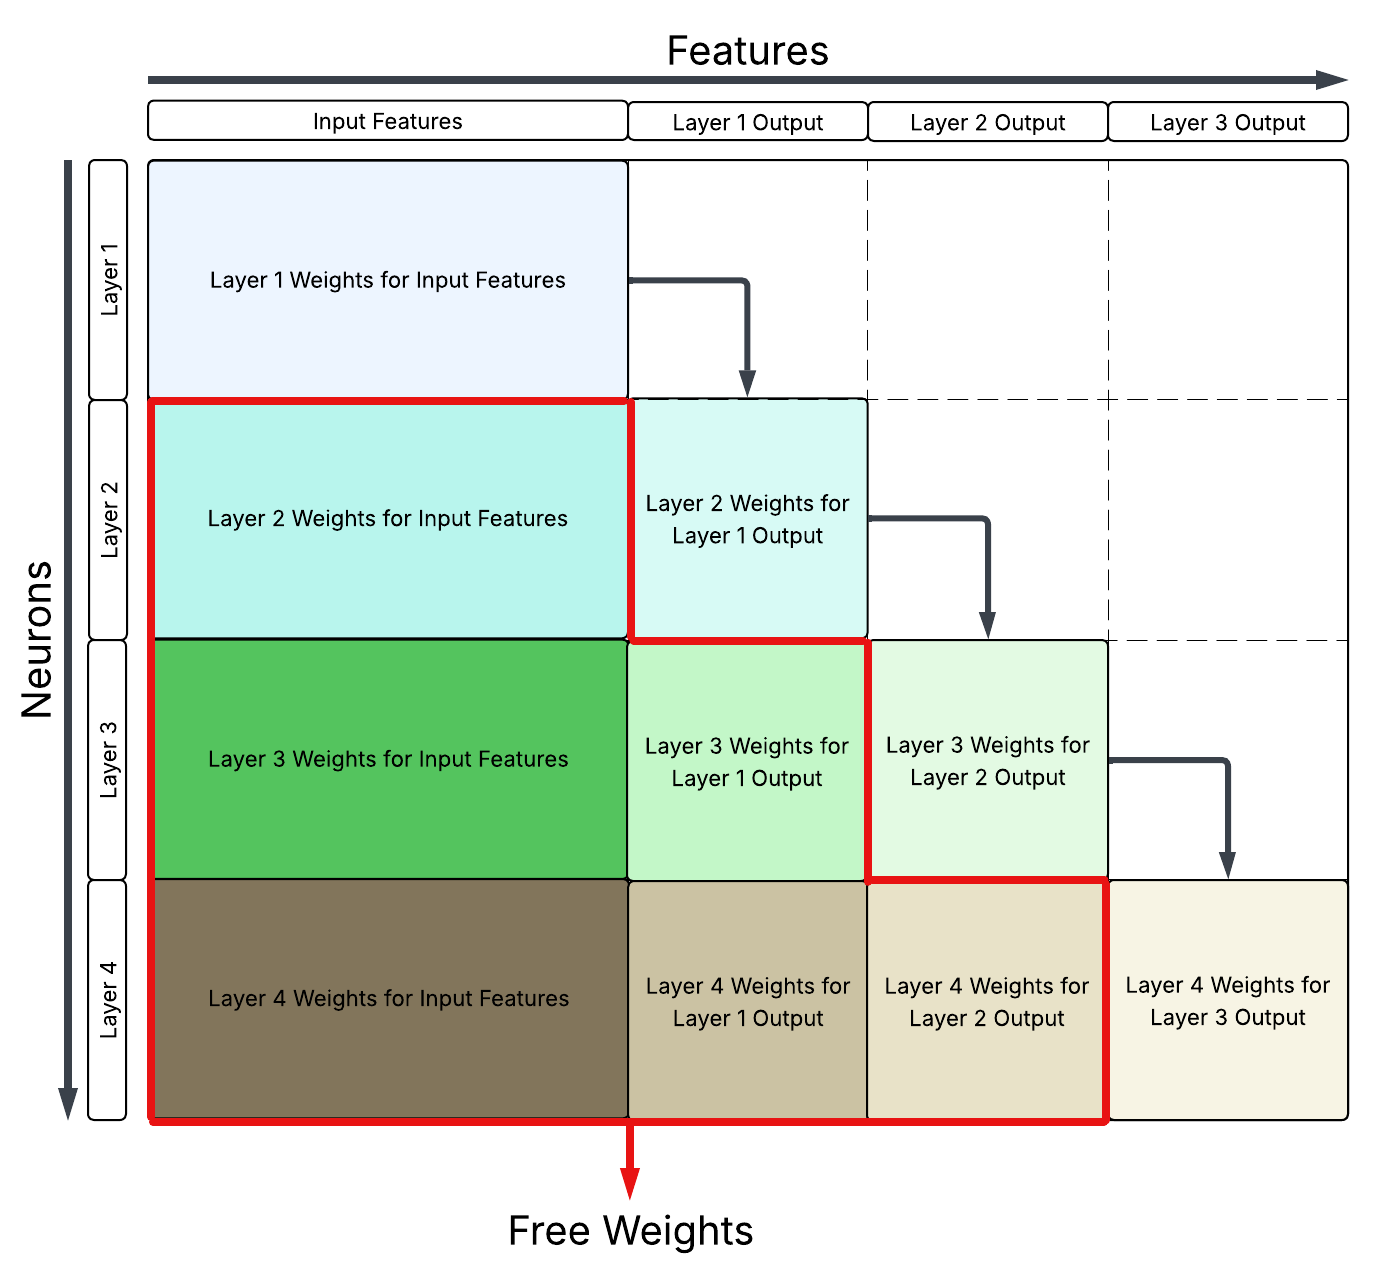
\includegraphics[width=0.7\textwidth]{Figures/Methodology/Free_Weights_SPN_Weights.png}
\caption{Illustration of a traditional MLP with Free Weights.}
\label{fig:fwSpn}
\end{figure}

\subsection{Maximal SPNs}

Additionally, by adding weights to the right side of the diagonal blocks, the weight matrix becomes a fully filled staircase pattern, with each "step" corresponding to a single neuron. This configuration not only maximizes the number of possible connections but also increases the layer count to match the total number of neurons, thereby minimizing the model’s throughput. Such a model, which achieves both maximal connectivity and maximal depth, is referred to as a Maximal SPN.

\begin{itemize}
    \item Time complexity of Maximal SPNs: $\mathcal{O}(n)$, since every neuron becomes its own layer
    \item Space complexity: Using $I$ as the number of features in the input data and $n$ as the number of neurons.
    \begin{align*}
    =\, & I + (I+1) + (I+2) + \dots + (I + n - 1) \\
    =\, & I \cdot (1 + 2 + \dots + (n-1)) \\
    =\, & I \cdot \frac{n(n-1)}{2} \\
    =\, & \mathcal{O}(I \cdot n^2)
    \end{align*}
\end{itemize}

\begin{figure}[h!]
\centering
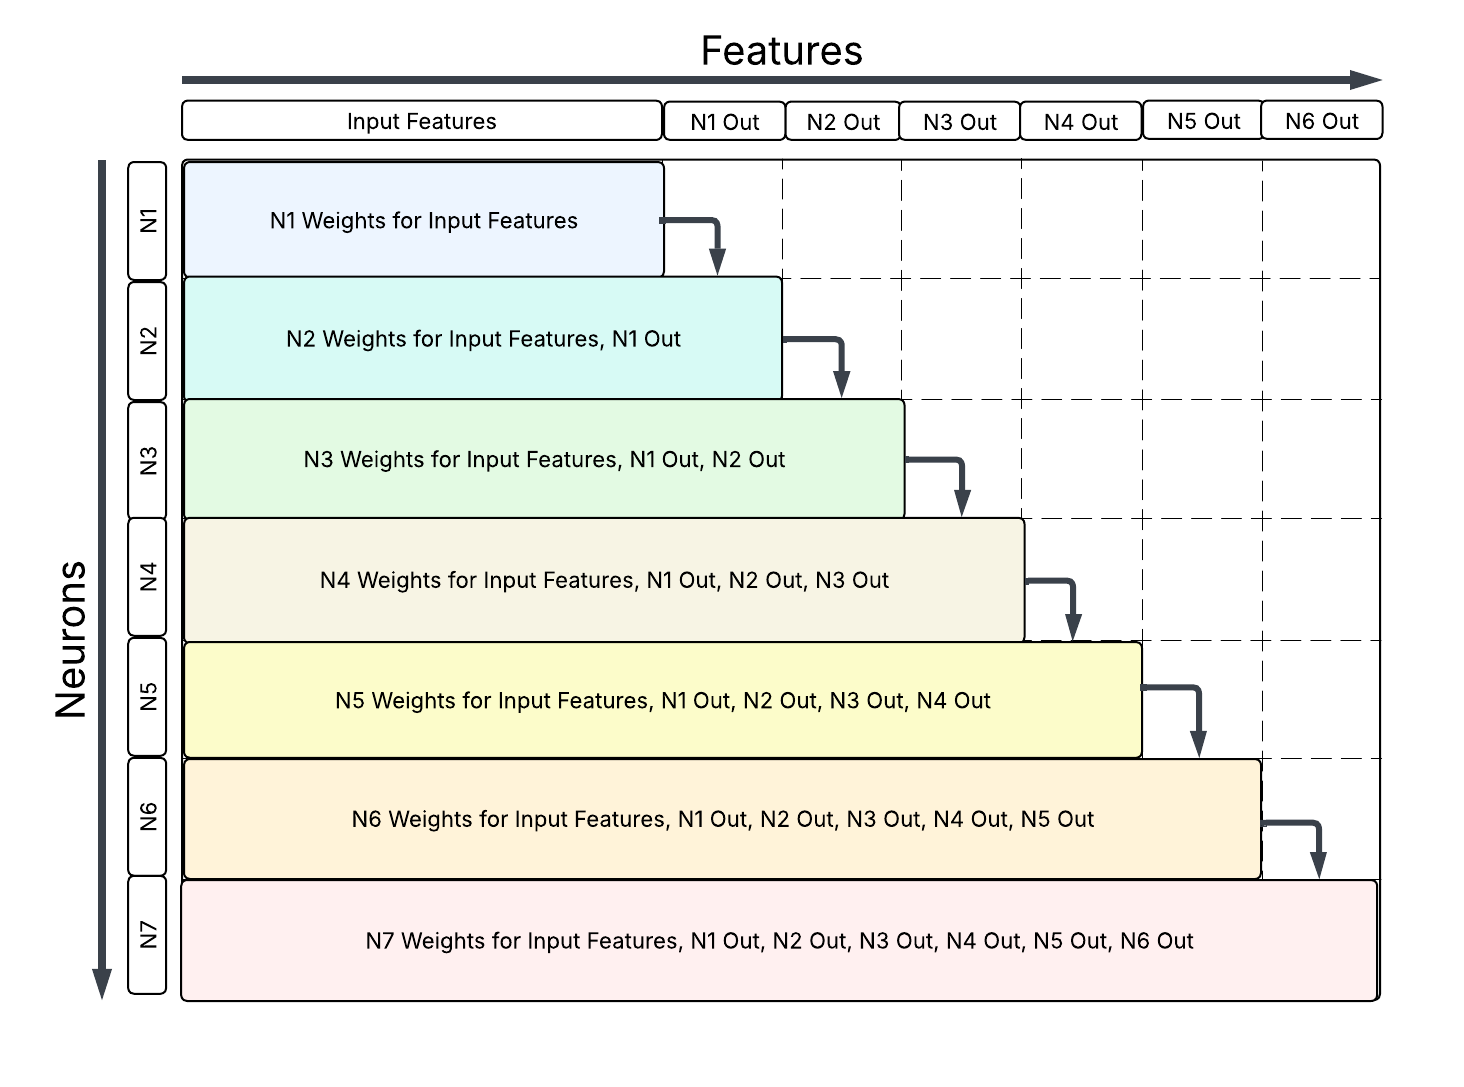
\includegraphics[width=0.7\textwidth]{Figures/Methodology/Neuron_Based_Maximal_SPN_Weights.png}
\caption{Illustration of a Maximal SPN.}
\label{fig:maxSpn}
\end{figure}

%-----------------------------------
%	SUBSECTION 2
%-----------------------------------

\subsection{Pruned Maximal SPNs}

Since maximal SPNs can have an excessive number of layers and consequently, poor throughput, one potential solution is \textbf{pruning}. The Lottery Ticket Hypothesis posits that over 90\% of weights in a network can be removed while still achieving performance comparable to the original network, suggesting the existence of a subnetwork within the initial network that is equally trainable~\cite{frankle2018lottery}.

Applying this principle, if we prune a maximal SPN, zeroing out selected weights on the rightmost edges of the staircase weight matrix, we effectively reduce dependencies between certain neurons as illustrated in Figure \ref{fig:pruningMaxSPN}. This reduction allows for the merging of independent neurons into shared layers, thus reintroducing parallelism to the network while maintaining its high expressiveness and capacity for learning complex data patterns.

\begin{figure}[h!]
\centering
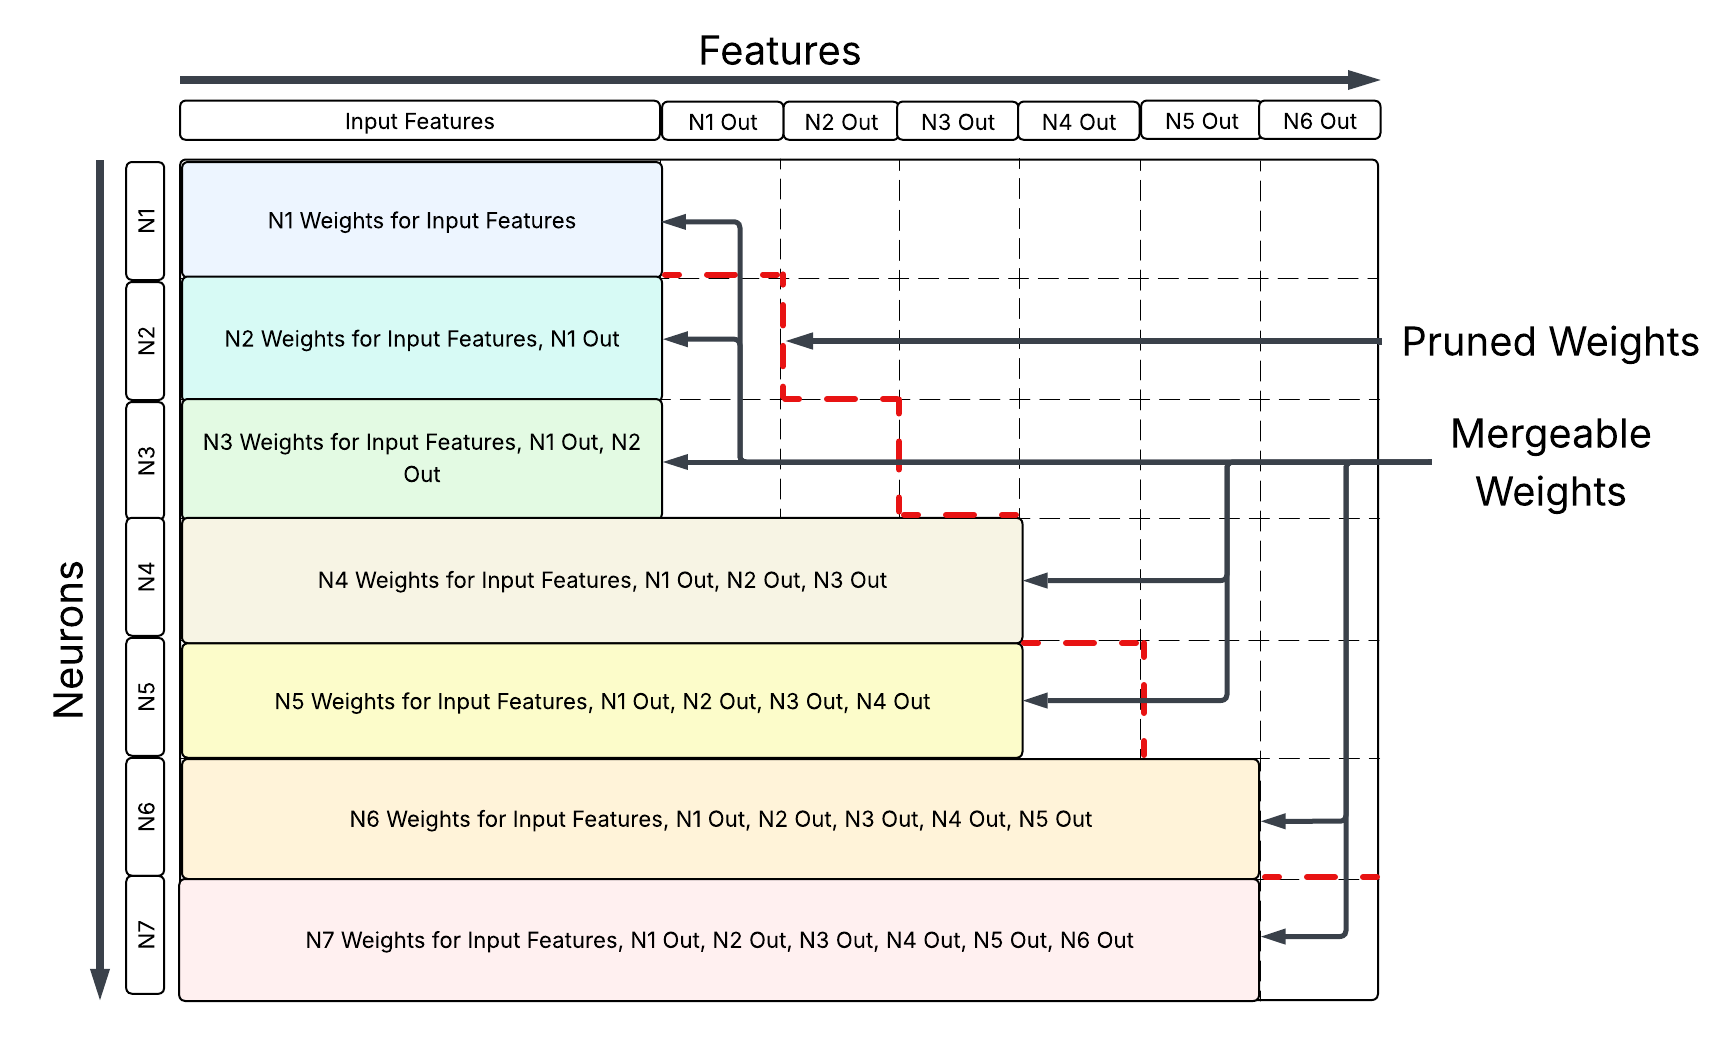
\includegraphics[width=0.7\textwidth]{Figures/Methodology/pruning_max_spn.png}
\caption{Pruning a Maximal SPN.}
\label{fig:pruningMaxSPN}
\end{figure}

The pruning strategy adopted in the current SPN framework is inspired by the Lottery Ticket Hypothesis and follows these steps:
\begin{enumerate}
    \item Train the original network to completion.
    \item Prune a fraction of the weights with the lowest magnitudes.
    \item Reset the remaining weights to their initial values.
    \item Repeat this process iteratively for several cycles.
\end{enumerate}

At the conclusion of this procedure, neurons that have become independent as a result of pruning are merged to reduce the overall layer count and improve throughput. It is important to note that merging is performed only after the entire pruning process has finished. Preliminary experiments revealed that merging neurons during pruning can alter the network's architecture in ways that negatively affect subsequent pruning steps, making the overall process less effective than waiting until pruning is complete.

\subsection{Minimal SPNs}

At the other end of the spectrum, if our goal is to minimize the number of layers while maximizing connectivity, we arrive at the concept of minimal SPNs. This involves organizing the network with as few layers as possible and enriching them with free weights.

Theoretically, the most minimal architecture would be a single perceptron, or for multiclass classification, a single layer with as many neurons as there are output classes ($o$). However, for this analysis, we assume a fixed total number of neurons ($n$) and seek to arrange them into layers to minimize throughput. This leads to two possible scenarios:

\begin{enumerate}
    \item When the total number of neurons equals the output size ($n = o$): Only a single output layer of size $o$ is possible, with no opportunity for cross-layer connections.
    \item When the total number of neurons exceeds the output size ($n > o$): The network can be organized into two layers: an output layer of size $o$ and a hidden layer with the remaining $n-o$ neurons. This configuration yields a minimal MLP, as illustrated in Figure \ref{fig:minMLP}. By introducing free weights, we transform it into a minimal SPN, depicted in Figure \ref{fig:minSpn}.
\end{enumerate}

\begin{itemize}
    \item Time complexity: $\mathcal{O}(1)$, since there can always be a maximum of two layers, the time complexity is constant.
    \item Space complexity: Using $I$ as the number of features in the input data and $n$ as the number of neurons.
    \begin{align*}
    =\, & I \cdot (n) + n \cdot o \\
    =\, & \mathcal{O}(I \cdot n)
    \end{align*}
\end{itemize}

\begin{figure}[h!]
    \centering
    \begin{minipage}[t]{0.48\textwidth}
        \centering
        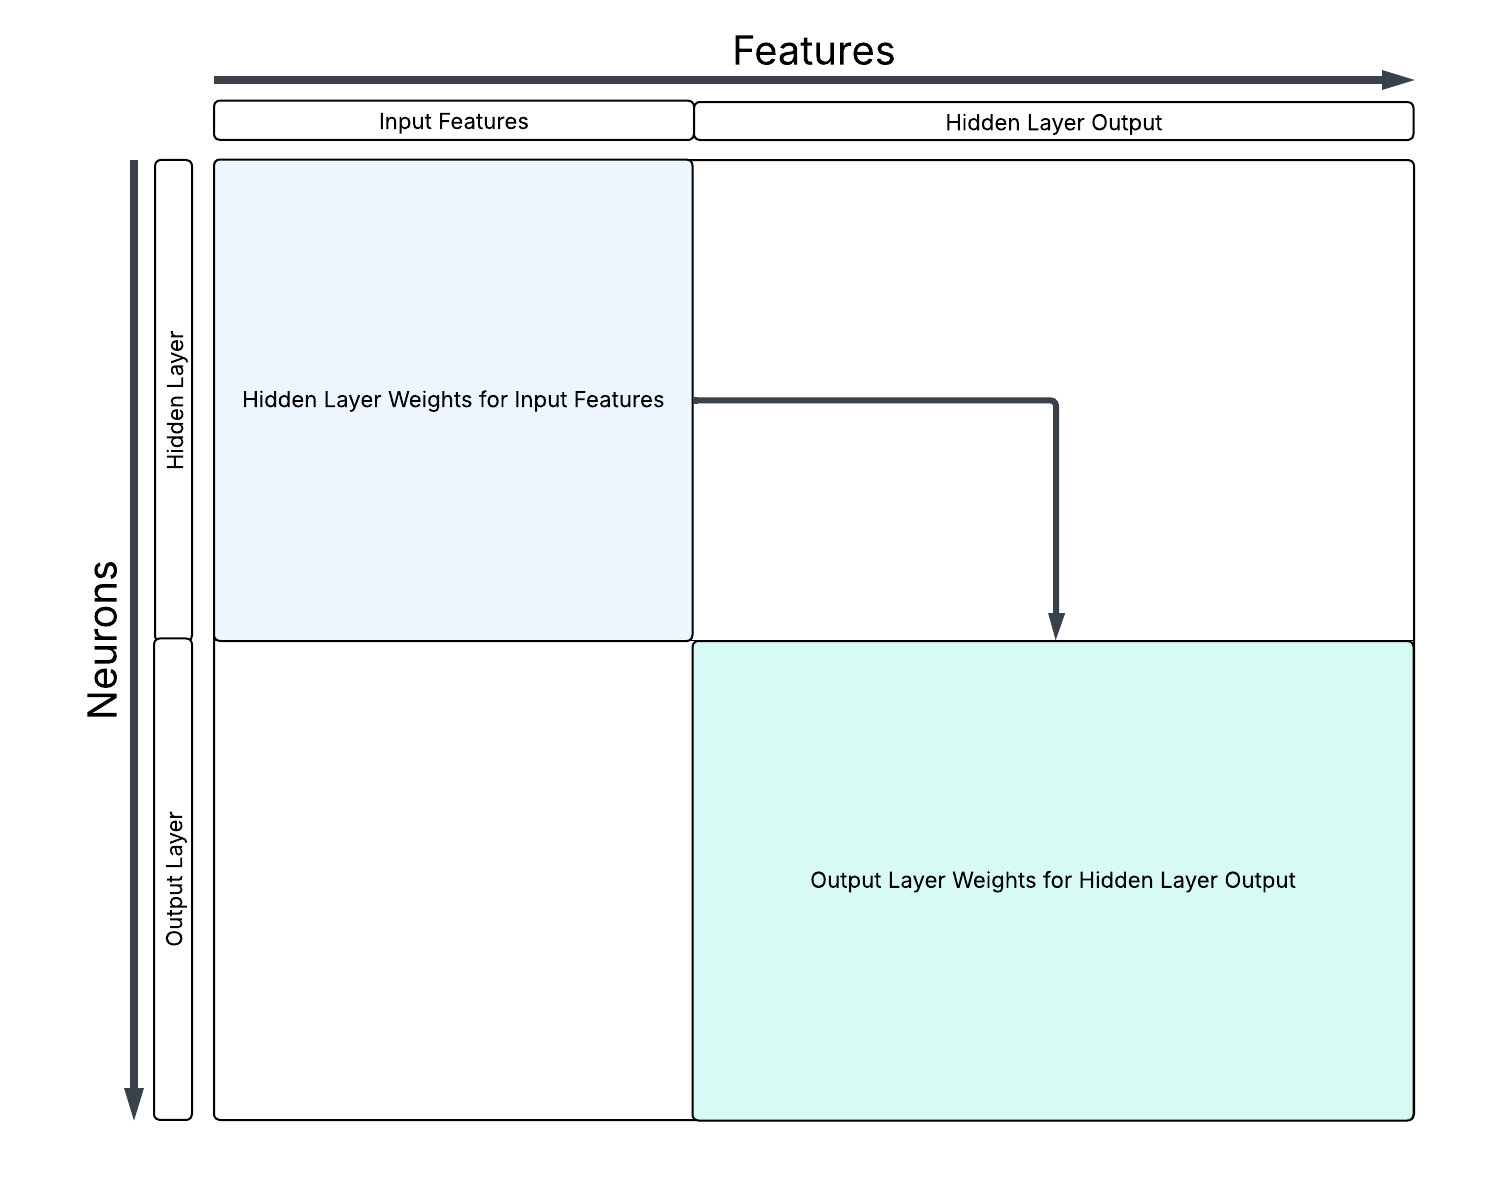
\includegraphics[width=\textwidth]{Figures/Methodology/Minimal_MLP_Weights.png}
        \caption{Minimal MLP.}
        \label{fig:minMLP}
    \end{minipage}%
    \hfill
    \begin{minipage}[t]{0.46\textwidth}
        \centering
        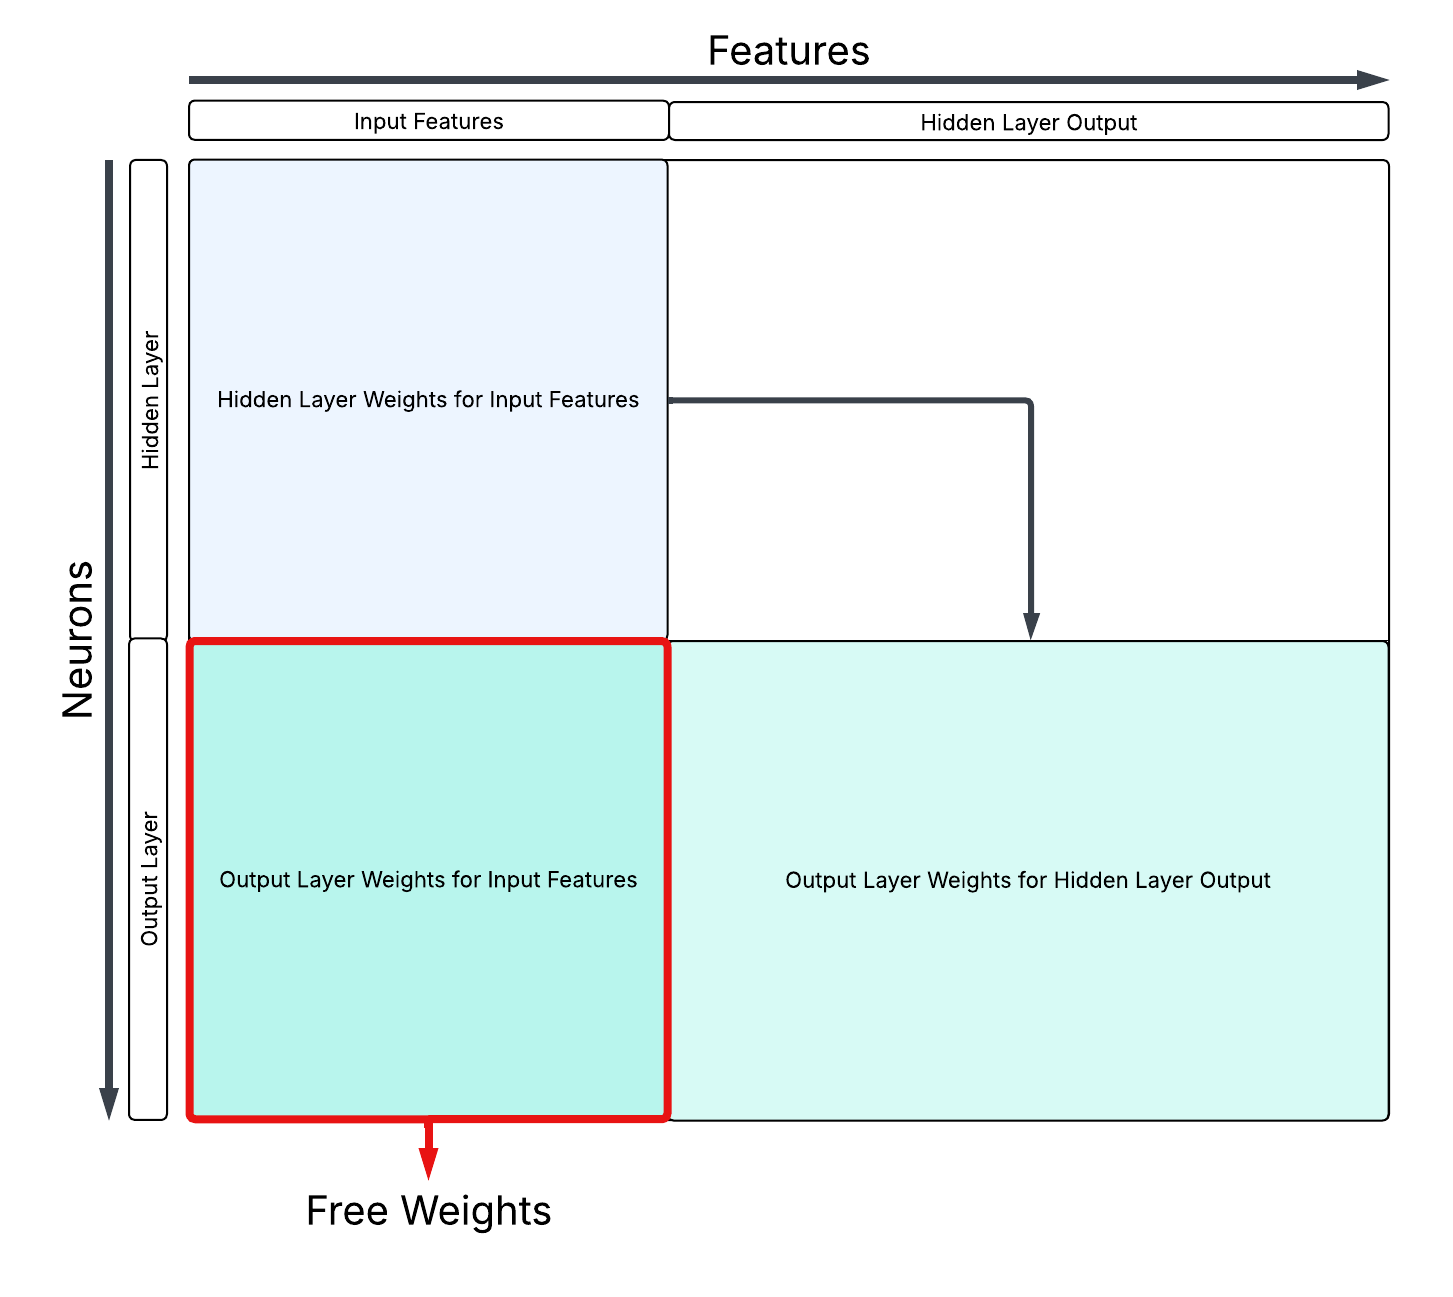
\includegraphics[width=\textwidth]{Figures/Methodology/Minimal_SPN_Weights.png}
        \caption{Minimal SPN.}
        \label{fig:minSpn}
    \end{minipage}
\end{figure}

\section{Implementation Approach}

In practice, there are three potential ways of designing the forward-propagation and backpropagation algorithms for SPNs. For all these approaches, the time and space complexity of implementing Maximal SPNs will be considered as they represent the worst case scenario.

\subsection{Object-based Representation with Partial Inputs}

One potential method to achieve the SPN framework is to have neurons, as independent objects, store partial inputs from sources that have completed their forward pass, while still waiting on outputs from other sources that haven't finished. Once a neuron receives all its necessary inputs, it performs its own forward pass and propagates its output to the subsequent neurons.
 
While this approach is conceptually simple and flexible, it is computationally expensive. Each neuron performs a storage and propagation step for every connection it has, leading to a large amount of redundancy. Even though the forward pass is only a single step once the inputs are complete, a worst-case scenario involves performing $n$ forward passes, where $n$ is the total number of neurons. Additionally, since each neuron stores its partial inputs, the outputs from a single neuron are duplicated for every neuron it propagates to. With each neuron also storing weights for every input, this method doubles the memory used compared to a traditional MLP network.

\begin{itemize}
    \item Time complexity: $\mathcal{O}(n^2)$.
    \item Space complexity: $\mathcal{O}(I \cdot n^2)$.
\end{itemize}

%----------------------------------------------------------------------------------------
%	SECTION 2
%----------------------------------------------------------------------------------------

\subsection{Sequential Representation}

In this approach, we describe the SPN using a list of weights, where every element in the list corresponds to the weights of a single neuron, exactly how it was illustrated in Figure \ref{fig:maxSpn}.
 
Such a network contains all possible connections for a given number of neurons. Therefore, any other network with the same number of neurons is a subnetwork of this complete network. To process this network, neurons are processed sequentially, starting from the first element in the list up to the last. For each step, the output of a neuron is appended to its input, providing the input for the subsequent neuron. By doing so, we eliminate the need to add partial inputs for each neuron individually. Instead, the same input can be compounded across the forward pass.

This approach assumes a maximum connection for every neuron. Disconnecting two neurons is achieved by zeroing out the weight value for the output neuron corresponding to the input. This method resembles traditional MLP pruning, where weight values are zeroed out instead of being removed entirely.

While this method eliminates the propagation step from every neuron to its subsequent neurons, it still requires each neuron to temporarily store its input during the backpropagation process. Therefore, this approach does not reduce space complexity.

\begin{itemize}
    \item Time complexity: $\mathcal{O}(n)$.
    \item Space complexity: $\mathcal{O}(I \cdot n^2)$.
\end{itemize}

\subsection{Block-based Representation}

When considering the weight matrix of a Maximal SPN, we can draw vertical lines at the edge of each neuron’s weight vector, forming vertical blocks within the matrix. The largest block, which is the first block, contains the weights corresponding to the input features, and subsequent blocks contain the weights for the output of each neuron as showin in Figure \ref{fig:blockMaxSpn}.
 
Rather than processing each neuron’s weight vector individually, this approach processes the network one block at a time. The top-most neuron’s forward pass is completed first, followed by calculating partial outputs for the remaining neurons. This method improves the time complexity by prioritizing the heaviest calculations (typically when the hardware is under lower load), and adds slight parallelization, as an input value is accessed only once, rather than repeatedly in a sequential approach.

This method is both energy and time-efficient, offering significant improvements over the previous approaches.

\begin{itemize}
    \item Time complexity: $\mathcal{O}(n)$.
    \item Space complexity: $\mathcal{O}(I \cdot n^2)$.
\end{itemize}

\begin{figure}[h!]
\centering
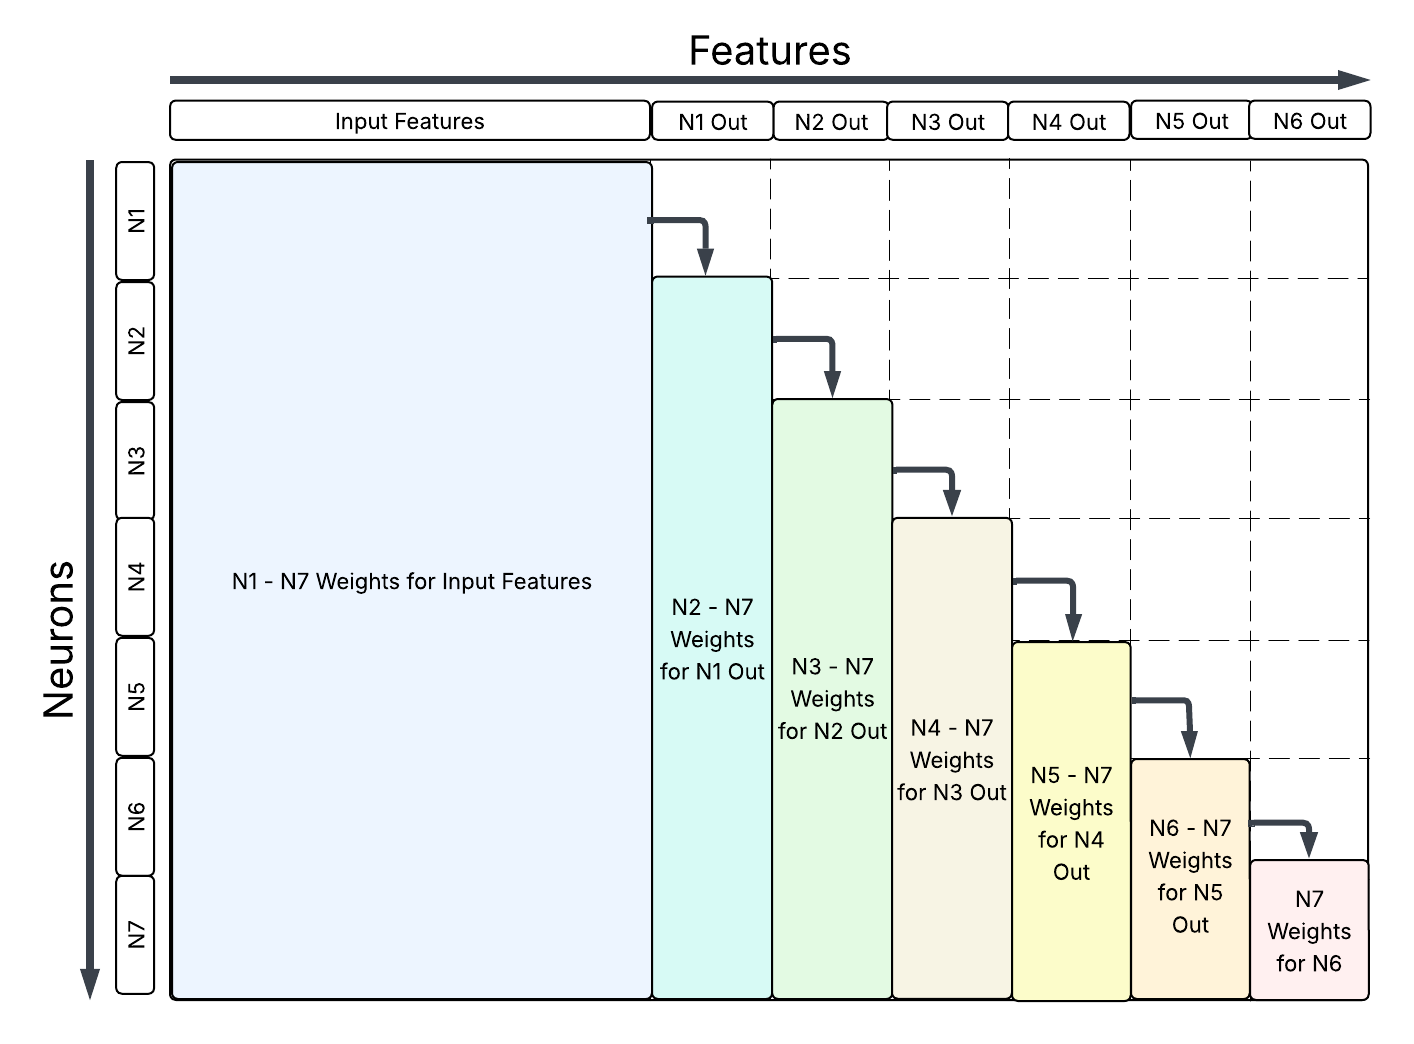
\includegraphics[width=0.8\textwidth]{Figures/Methodology/Block_Based_Maximal_SPN_Weights.png}
\caption{Illustration of a block based Maximal SPN.}
\label{fig:blockMaxSpn}
\end{figure}

\subsection{Summary}

The performance difference between the sequential and block-based approaches is minimal, as both exhibit the same overall time complexity. Their relative efficiency primarily depends on the underlying hardware. The block-based approach front-loads the computational burden by handling the most demanding calculations first, while the sequential approach distributes the workload more evenly across all steps. Depending on the hardware and the specific model architecture, one approach may be preferable over the other.

\begin{table}[h!]
\centering
\caption{Comparison of time and space complexities for the implementation approaches.}
\begin{tabular}{|l|l|l|}
\hline
\textbf{Approach}    & \textbf{Time Complexity} & \textbf{Space Complexity} \\
\hline
Object Based          & $\mathcal{O}(n^2)$        & $\mathcal{O}(I \cdot n^2)$        \\
Sequential          & $\mathcal{O}(n)$        & $\mathcal{O}(I \cdot n^2)$       \\
Block Based              & $\mathcal{O}(n)$        & $\mathcal{O}(I \cdot n^2)$        \\
\hline
\end{tabular}
\label{tab:approachescomplexityComparison}
\end{table}

In this thesis, the sequential method was chosen for its balanced workload distribution; with larger models, the block-based approach could potentially overwhelm hardware resources at the outset, resulting in slower performance. Ultimately, a hybrid strategy that combines elements of both approaches may offer the greatest efficiency.